%% Document-wide settings.
\documentclass[letterpaper]{article}
\title{Poaky documentation}
\author{Thomas HOULLIER} 

\usepackage[colorlinks=true, allcolors=blue,
            hyperfootnotes=false,
            pdfauthor={Thomas HOULLIER},
            pdftitle={Poaky documentation},
	    pdfkeywords={Optical design, Raytracing, C++}]
            {hyperref} % Links for ref/cite.

%% Loading packages
\usepackage{amsmath} % For cases in equations.
\usepackage{amsfonts} % For maths sets.
\usepackage{amssymb} % Square symbol for QED
\usepackage{physics} % For \abs{} and \norm{}.
\usepackage[inkscapelatex=false]{svg} %svg graphics
\usepackage{siunitx} % units formatting

\usepackage[backend=biber,style=numeric,citestyle=numeric-comp,maxcitenames=99,dateabbrev=false]{biblatex}
\addbibresource{biblio.bib}
\usepackage{setspace} % Bibliography spacings
\DeclareSourcemap{
  \maps[datatype=bibtex]{
    \map[overwrite]{
      \step[fieldsource=doi, final]
      \step[fieldset=url, null]
      \step[fieldset=eprint, null] }}}
\setcounter{biburllcpenalty}{7000} % break long url in bibliography
\setcounter{biburlucpenalty}{8000}
\renewcommand*{\bibfont}{\footnotesize} % bibliography font size
% Format of biblatex urldate in the bibliography.
\DeclareFieldFormat{urldate}{%
  Visited on \thefield{urlday}\addspace%
  \mkbibmonth{\thefield{urlmonth}}\addspace%
  \thefield{urlyear}\isdot}
\usepackage[ruled,vlined]{algorithm2e} % Algorithms.
\DontPrintSemicolon
\SetKwInOut{Input}{Input}\SetKwInOut{Output}{Output}
\usepackage{mathtools} % Ceiling function.
\usepackage{outlines} % Nest lists.
\usepackage{interval} % Writing intervals.
\usepackage[font={footnotesize,sf}]{caption} %Caption for figures in minipages.
\usepackage{floatrow}
% Figure captions always below. Figures always centered.
\floatsetup[figure]{capposition=bottom,objectset=centering}
\usepackage{wrapfig} %Wrapping figure with text.
\usepackage{stmaryrd} % Double brackets for integers interval.
\usepackage{doi} % Hyperlink DOI
\usepackage{etoolbox} %Ragged right bibliography.
\usepackage{color, colortbl} % Coloring rows in tables.
\usepackage{subcaption} % Subfigures.
\usepackage{pdfpages} % Include PDF pages.
\usepackage{epigraph} % Quotations at beginning of chapters.
\setlength\epigraphwidth{.8\textwidth}
\usepackage[acronym,nonumberlist,nogroupskip,nopostdot]{glossaries} % Glossary for acronyms.
\renewcommand*{\glstextformat}[1]{\textcolor{black}{#1}} % No color on links for abbrev.

\DeclarePairedDelimiter{\ceil}{\lceil}{\rceil} % Ceiling function.
\DeclarePairedDelimiter{\floor}{\lfloor}{\rfloor} % Floor function.

\DeclareMathOperator*{\argmin}{argmin}

\setcounter{tocdepth}{3} % Table of content depth
\setcounter{secnumdepth}{3} % Section numbering depth

% Non-breaking around footnotes.
\makeatletter
\let\Footnote\footnote
\def\pst@@killglue{\unskip\ifdim\lastskip>\z@\expandafter\pst@@killglue\fi}
\def\footnote{\pst@@killglue\Footnote}
\makeatother

% More space below equations
\appto\normalsize{\belowdisplayshortskip=\belowdisplayskip}

% Rewrite month codes in bibliography
\DeclareSourcemap{
  \maps[datatype=bibtex]{
    \map[overwrite]{
      \step[fieldsource=month, match=\regexp{\A(j|J)an(uary)?\Z}, replace=1]
      \step[fieldsource=month, match=\regexp{\A(f|F)eb(ruary)?\Z}, replace=2]
      \step[fieldsource=month, match=\regexp{\A(m|M)ar(ch)?\Z}, replace=3]
      \step[fieldsource=month, match=\regexp{\A(a|A)pr(il)?\Z}, replace=4]
      \step[fieldsource=month, match=\regexp{\A(m|M)ay\Z}, replace=5]
      \step[fieldsource=month, match=\regexp{\A(j|J)un(e)?\Z}, replace=6]
      \step[fieldsource=month, match=\regexp{\A(j|J)ul(y)?\Z}, replace=7]
      \step[fieldsource=month, match=\regexp{\A(a|A)ug(ust)?\Z}, replace=8]
      \step[fieldsource=month, match=\regexp{\A(s|S)ep(tember)?\Z}, replace=9]
      \step[fieldsource=month, match=\regexp{\A(o|O)ct(ober)?\Z}, replace=10]
      \step[fieldsource=month, match=\regexp{\A(n|N)ov(ember)?\Z}, replace=11]
      \step[fieldsource=month, match=\regexp{\A(d|D)ec(ember)?\Z}, replace=12]}}}

% Footnotes marker color
\renewcommand\thefootnote{\textcolor{blue}{\arabic{footnote}}}

\pdfsuppresswarningpagegroup=1 % Silence warnings about pagegroups for figures.
\pdfminorversion=6 % PDF version 1.6 since we include articles in 1.6.

% Allow an extra pass to fix overfull hboxes by allowing more whitespace.
\emergencystretch=1em

% Page numbering and copyright notice.
\usepackage{fancyhdr}
\usepackage{lastpage}

\fancypagestyle{FirstPage}{
\fancyhf{} % Clear footer.
\rfoot{\thepage \hspace{1pt} of \pageref*{LastPage}}
\renewcommand{\headrulewidth}{0pt} % Remove rule at top of page
\lfoot{\href{https://creativecommons.org/licenses/by/4.0/}
       {\includesvg[inkscapelatex=false,height=14pt]{images/ccby.svg}}}
\lhead{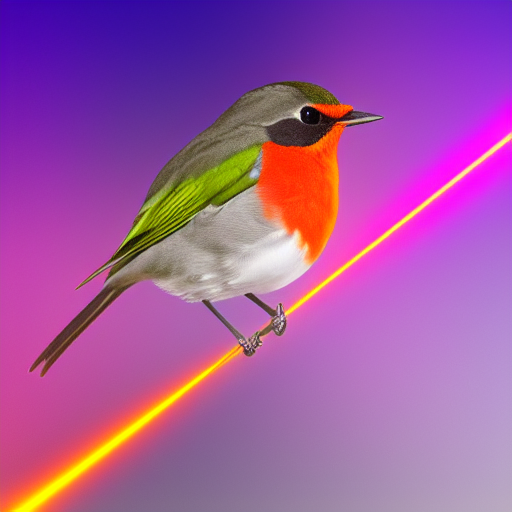
\includegraphics[height=64pt]{images/robintrace-logo.png}}
\chead{RobinTrace}
}

\fancypagestyle{plain}{
\fancyhf{} % Clear footer.
\rfoot{\thepage \hspace{1pt} of \pageref*{LastPage}}
\renewcommand{\headrulewidth}{0pt} % Remove rule at top of page
}

% Version history
\usepackage{vhistory}

% Keywords
\providecommand{\keywords}[1]{\textbf{Keywords --} #1}

% Glossary
\makeglossaries
\loadglsentries{glossary/glossary.tex}

\usepackage{fontawesome} %inline icons
\usepackage{xcolor}
\usepackage{listings} % Code listings
\definecolor{codeback}{rgb}{0.99,0.99,0.98}
\definecolor{codecomment}{HTML}{0588fc}
\definecolor{codekeyword}{HTML}{af5f00}
\definecolor{codestring}{HTML}{ffa07a}
\lstdefinestyle{mystyle}{
  backgroundcolor=\color{codeback},
  commentstyle=\color{codecomment},
  keywordstyle=\color{codekeyword},
  stringstyle=\color{codestring},
  basicstyle=\ttfamily\footnotesize,
  breakatwhitespace=false,         
  breaklines=true,                 
  captionpos=b,                    
  keepspaces=true,                 
  numbers=left,                    
  numbersep=5pt,                  
  showspaces=false,                
  showstringspaces=false,
  showtabs=false,                  
  tabsize=2}
\lstset{style=mystyle}

\usepackage[capitalise,nameinlink]{cleveref} % Include eg. "Fig." in front of figures.
\crefname{algorithm}{Alg.}{Algs.}
\crefname{table}{Tab.}{Tabs.}
\crefname{equation}{Eq}{Eqs.}
% Equation cross-references.
%\creflabelformat{equation}{#2#1#3}
\crefformat{equation}{(#2Eq.\thinspace#1#3)}

% No parentheses in equation labels.
%\newtagform{noparen}{}{}
%\usetagform{noparen}



% Document
\begin{document}
\frenchspacing
\date{v1.0 -- \today}
\maketitle
\thispagestyle{FirstPage}

\begin{abstract}
We document the development of Poaky, a piece of software for raytracing
through optical systems. Poaky is implemented in C++.
\end{abstract}

\keywords{Optical design, Raytracing, C++}

\begin{versionhistory}
\vhEntry{1.0}{\today}{TH}{creation}
\end{versionhistory}
\setcounter{table}{0} % Reset the table counter.

\tableofcontents
\printglossary[type=\acronymtype,style=index]
\pagestyle{plain}
\section{Scope}
Poaky deals with tracing rays of light through optical systems,
under the laws of geometrical optics. It allows defining an optical system
with surfaces propagates rays through the system. Poaky reports the
state of rays at given optical surfaces.

The following optical design related items are left out:
\begin{itemize}
\item Phase computation: The rays are purely described by their trajectory.
\item Building objective functions and constraints: This belongs in a higher
layer which uses the states of rays to build performance criteria.
\item Optimization: This is an even higher layer than objective functions.
\item Ray-aiming: We can implement this on top of the current program.
\item User-level optical system definition: The optical system defined
      by the user does not use the same formalism as that of the current
      program.
\end{itemize}

\textcolor{red}{Whether ray-aiming and higher functions will be included
in the current repository or another is not yet decided.}

\section{Architecture}
The software architecture follows an object-oriented, bottom-up approach.
From the lowest level of abstraction to highest, we may describe the
major objects as follows:

\begin{itemize}
\item \lstinline{ray}: Rays are the most fundamental data object in the
program.  Each ray is represented by $(x, y, z)$ local coordinates and $(l, m,
n)$ local direction cosines.
\item \lstinline{rop} (ray operations): These are low-level operations
modifying \lstinline{rays}.  They are used by \lstinline{low-level surfaces}.
They may be common to multiple surface types. A typical example is the
intersection of a ray with a sphere.
\item \lstinline{lpart} (low-level part): These are low-level objects which
are ordered in succession. These are groupings of \lstinline{rop}
which correspond to common optical design surface elements. There are two
fundamental subtypes:
\begin{itemize}
\item \lstinline{surf} (surface): This group of operations takes a ray starting
from the local surface plane and outputs rays also in the local coordinate
system at the computed positions.
\item \lstinline{tfr} (transfer): These operations take rays from a starting
surface coordinate system and propagate them in straight lines to another
plane. The output rays are expressed in a new local surface plane.
\end{itemize}
\item \lstinline{bun} (ray bundles): These are arrays of \lstinline{ray}. They
include some higher level utilities such as tracking and reporting the state of
rays.
\item \lstinline{lsys} (low-level system): This is a succession of
\lstinline{lpart}.
\item \lstinline{ltrac} (low-level tracer): This object holds both a
\lstinline{lsys} and a \lstinline{bun}. It is responsible for applying
operations and reporting the state of the rays to higher parts of the program.
\end{itemize}

This architecture is summarized informally using a diagram
(\cref{fig:arch-overview}).

\begin{figure} 
\includesvg[width=.9\textwidth]{images/arch/overview/overview.svg}
\caption{\label{fig:arch-overview} Architecture overview.}
\end{figure}

\section{Functional description}

\textcolor{red}{TODO: \begin{itemize}
\item Detail the behavior of a minimal set of components for
only 3D mirrors.
\end{itemize}}

\subsection{ray}

\textcolor{red}{xyzlmn description, short rationale on the fact rays hold
minimal information and their meaning depends on context.
Error codes for each ray?}

\subsection{rop}

\textcolor{red}{
\begin{itemize}
\item ray/plane intersection
\item ray/sphere intersection
\item ray reflection on a plane mirror
\item ray reflection on spherical mirror
\item transfer operation
\end{itemize}
Explain rationale to have the most specialized operations possible here.
And why operations are dissociated from lpart.}

\subsection{lpart}

\subsubsection{tfr}

\subsubsection{surf}
\textcolor{red}{
\begin{itemize}
\item Plane (which does nothing)
\item Plane mirror
\item Spherical mirror
\end{itemize}}

\section{Tests and benchmarks}
We document what tests are performed on the components of the software.
We also detail a representative performance report.

\subsection{Tests}

\subsection{Performance report}
A performance report helps both the user and developer understand the strengths
and weaknesses of the software computations.


\appendix
\cleardoublepage

%% \include{appendices}

\apptocmd{\thebibliography}{\raggedright}{}{}
\begingroup
\setstretch{0.6}
\setlength\bibitemsep{0pt}
\printbibliography
\endgroup
\end{document}
